% Author: Nikita Moiseev <xmoise01@stud.fit.vutbr.cz>
% Author: Maksim Kalutski <xkalut00@stud.fit.vutbr.cz>
% Author: Elena Marochkina <xmaroc00@stud.fit.vutbr.cz>
% Author: Nikita Pasynkov <xpasyn0034@stud.fit.vutbr.cz>


\documentclass[a4paper, 11pt]{article}


\usepackage[czech]{babel}
\usepackage[utf8]{inputenc}
\usepackage{geometry} \geometry{verbose,a4paper,tmargin=2cm,bmargin=2cm,lmargin=2.5cm,rmargin=1.5cm}
\usepackage{times}
\usepackage{geometry}
\usepackage{verbatim}
\usepackage{enumitem}
\usepackage{graphicx} % insert picture
\usepackage[unicode]{hyperref}
\usepackage[table,xcdraw]{xcolor}
\documentclass[xcolor=table]{beamer}
\hypersetup{
	colorlinks = false,
	hypertexnames = false,
	citecolor = blue
}
\usepackage{pdflscape}

\begin{document}
	%% Title page %%
	\begin{titlepage}
		\begin{center}
			\includegraphics[width=0.77\linewidth]{fit_logo.png} \\

			\vspace{\stretch{0.382}}

			\Huge{Projektová dokumentace} \\
			\LARGE{\textbf{Implementace překladače imperativního jazyka IFJ22}} \\
			\Large{Tým \textbf{xmoise01}, varianta \textbf{BVS}}
			\vspace{\stretch{0.7}}
		\end{center}

		\begin{minipage}{0.4 \textwidth}
			{\Large \today}
		\end{minipage}
		\hfill
		\begin{minipage}[r]{0.6 \textwidth}
			\Large
			\begin{tabular}{l l l}
				\textbf{Nikita Moiseev} & \textbf{(xmoise01)} & \quad 25\,\% \\
				Maksim Kalutski & (xkalut00) & \quad 25\,\% \\
				Elena Marochkina & (xmaroc00) & \quad 25\,\% \\
				Nikita Pasynkov & (xpasyn00) & \quad 25\,\% \\
			\end{tabular}
		\end{minipage}
	\end{titlepage}



	% Obsah %
	\pagenumbering{roman}
	\setcounter{page}{1}
	\tableofcontents
	\clearpage



	% Úvod %
	\pagenumbering{arabic}
	\setcounter{page}{1}

	\section{Úvod}
	Cílem projektu bylo vytvořit program v~jazyce~C, který načte zdrojový kód zapsaný ve zdrojovém jazyce IFJ22,
	jenž je zjednodušenou podmnožinou jazyka PHP a~přeloží jej do cílového jazyka IFJcode22 (mezikód).

	Program funguje jako konzolová aplikace, které načítá zdrojový program ze standardního vstupu a~generuje
	výsledný mezikód na standardní výstup nebo v~případě chyby vrací odpovídající chybový kód.



	% Návrh a implementace %
	\section{Návrh a~implementace}

	Projekt jsme sestavili z~několika námi implementovaných dílčích částí, které jsou představeny v~této kapitole.
	Je zde také uvedeno, jakým způsobem spolu jednotlivé dílčí části spolupracují.


	\subsection{Lexikální analýza}

	Při tvorbě překladače jsme začali implementací lexikální analýzy. Hlavní funkce této analýzy je \texttt{get\_next\_token},
	pomocí níž se čte znak po znaku ze zdrojového souboru a~převádí na strukturu \texttt{token}, která se skládá z~typu a~hodnoty.
	Typy tokenu jsou \texttt{EOF}, speciální znaky, speciální závorky PHP, identifikátory, klíčová slova, datové typy a~také aritmetické, relační a logické operátory a operátor přiřazení a~ostatní znaky, které mohou být použity v~jazyce IFJ2022.
	Hodnota atributu je
	\texttt{value}. Pokud je typ tokenu identifikátor, pak bude atribut daný identifikátor,
	když by byl typ tokenu klíčové slovo, přiřadí atributu dané klíčové slovo, pokud číslo, atribut bude ono číslo. S~takto vytvořeným tokenem poté pracují další analýzy.

	Celý lexikální analyzátor je implementován jako deterministický konečný automat podle předem vytvořeného diagramu
	\ref{figure:fa_graph}. Konečný automat je v~jazyce C~jako jeden nekonečně opakující se \texttt{switch}, kde každý případ
	\texttt{case} je ekvivalentní k~jednomu stavu automatu. Pokud načtený znak nesouhlasí s~žádným znakem, který jazyk povoluje,
	program je ukončen a~vrací chybu 1 \texttt{LEXICAL ERROR CODE 1}. Jinak se přechází do dalších stavů a~načítají se další znaky, dokud nemáme hotový jeden
	token, který potom vracíme a~ukončíme tuto funkci.


	\subsection{Syntaktická analýza}

	Nejdůležitější částí celého programu je syntaktická analýza. Syntaktická analýza je implementována v souboru
	\texttt{syntax\_analyzer.c}, a její rozhraní pro implementaci v \texttt{syntax\_analyzer.h}.

	Syntaktická analýza je implementována pomocí rekurzívního sestupu na základě LL gramatiky - Tabulka ~\ref{table:ll_gramatika}. Syntaktický
	analyzátor zpracovává všechny části LL gramatiky na výrazy podle pravidel v LL - tabulce - Tabulka ~\ref{table:ll_table}. Úkolem
	syntetického analyzátoru je sestavit abstraktní syntaktický strom na základě seznamu tokenů. Strom je postaven
	tak, že je nastavena priorita operací a ve výsledku můžeme načtením tohoto stromu spustit kód v
	požadovaném pořadí. Pokud je nalezena chyba, překladač dokončí kontrolu, vymaže alokovanou paměť
	a zobrazí chybovou hlášku na standartní chybový vstup. Syntaktický analyzátor nijak neupravuje tokeny a všechny
	chyby jsou detekovány až v průběhu sémantické analýzy. Po vytvoření abstraktního syntaktického stromu
	syntaktický analyzátor přejde do další fáze sémantické analýzy.

	Príklady stromu pro syntaktickou analýzu jsou uvedeny na obrázkéch~\ref{figure:ast_example1}-~\ref{figure:ast_example4}.

	\newpage

	\begin{figure}[!ht]
		\centering
		\includegraphics[width=1\linewidth]{assign.pdf}
		\caption{Abstraktní syntaktický strom přirážení proměnných}
		\label{figure:ast_example1}
	\end{figure}

    \begin{figure}[!ht]
		\centering
		\includegraphics[width=1\linewidth]{if.pdf}
		\caption{Abstraktní syntaktický strom větvení}
		\label{figure:ast_example2}
	\end{figure}

    \begin{figure}[!ht]
		\centering
		\includegraphics[width=1\linewidth]{func_dec.pdf}
		\caption{Abstraktní syntaktický strom deklarací funkcí}
		\label{figure:ast_example3}
	\end{figure}

    \begin{figure}[!ht]
		\centering
		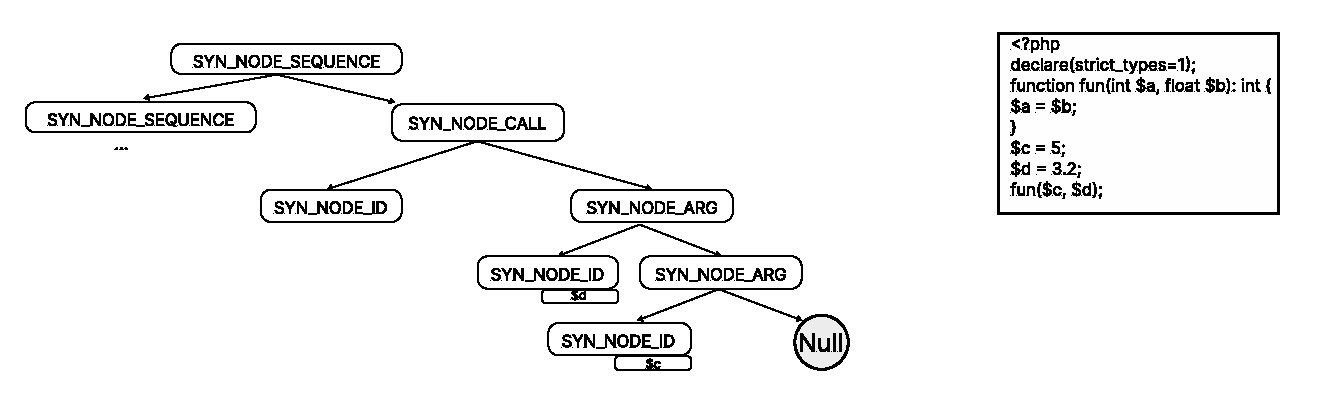
\includegraphics[width=1\linewidth]{fun_call.pdf}
		\caption{Abstraktní syntaktický strom volání funkcí}
		\label{figure:ast_example4}
	\end{figure}
    \newpage

	\subsection{Sémantická analýza}
	Sémantická analýza je implementována v souboru \texttt{semantic\_analyzer.c} a její rozhraní pro implementaci
	v \texttt{semantic\_analyzer.h}.

    Sémantický analyzátor pracuje s abstraktním syntaktickým stromem, který
	vytvořil syntaktický analyzátor. Úkolem sémantického analyzátoru je kontrola sémantické správnosti zdrojového
	programu: kontrola deklarací, datových typů, seznamů parametrů apod. a to pomocí kontroly datových typu.

    K tomu využívá datové struktury a funkce pro sémantické kontroly. Pokud při kontrole je nalezena chyba, překladač dokončí
	kontrolu, vymaže alokovanou paměť a zobrazí chybovou hlášku na standartní chybový vstup.

    V souboréch \texttt{symtable.c} a \texttt{symtable.h} je uložená tabulka symbolů.

    Tabulka symbolů je binární vyhledávací strom, který obsahuje informace o všech identifikátorech kódu. Tabulka symbolů se skládá jak z globálního stromů (pro všechny globální proměnné), tak z lokálních stromů (pro argumenty a lokální proměnné funkcí).


    Tabulka symbolů je uložena a okamžitě použita v sémantické analýze a~slouží ke kontrole, zda daný identifikátor existuje a~zda souhlasí jeho datový typ, případně návratová hodnota.


	Příklad stromu pro tabulku symbolů je uveden na obrázku~\ref{figure:sem_anal_example}.

	\begin{figure}[!ht]
		\centering
		\includegraphics[width=1\linewidth]{sem_anal.pdf}
		\caption{Tabulka symbolů}
		\label{figure:sem_anal_example}
	\end{figure}

    \subsection{Optimalizáce kódu}
    Optimalizáce kódu je implementováné v souboru \texttt{optimiser.c} a jeho rozhraní pro implementaci v souboru \texttt{optimiser.h}.

    Optimalizáce kódu pracuje s abstraktním syntaktickým stromem a mění ho.

    Optimalizátor kódu se spustí ihned po sémantické analýze a před vygenerováním kódu.

    Optimalizátor kódu provádí následující hlavní akce:
    \begin{enumerate}
        \item Optimalizuje matematické výrazy (například \texttt{\$a = 5 + 9/3; -> \$a = 8;})
        \item Přiřazování a změna hodnoty proměnné během programu
        \item Optimalizuje nedosažitelné smyčky while a if
        \item Odstraňuje nepoužívané proměnné
    \end{enumerate}

	\subsection{Generování cílového kódu}
    Generování cílového kódu je implementováné v souboru \texttt{code\_generator.c} a jeho rozhraní pro implementaci
	v \texttt{code\_generator.h}.  Generování kódu pracuje s abstraktním syntaktickým stromem po optimalizáce kódu.

    Generování cílového kódu znamená generování mezikódu IFJcode22. Kód je generován na standardní výstup po dokončení všech analýz.

	Na začátku generování jsou inicializovány potřebné datové struktury (které jsou na závěr uvolněny), vygenerována hlavička mezikódu, která zahrnuje potřebné náležitosti pro korektní interpretaci mezikódu a~skok do hlavního těla programu. Poté jsou vygenerovány vestavěné funkce, které jsou zapsány přímo v~jazyce IFJcode22.

     Každá funkce mezikódu IFJcode22 je tvořena návěštím ve tvaru \texttt{\$generate\_funkce}.

    Pak se spouští parser syntaktického stromu, dokud není nalezen jeden z uzlů: \texttt{SYN\_NODE\_ASSIGN, \\SYN\_NODE\_KEYWORD\_IF, SYN\_NODE\_KEYWORD\_WHILE, SYN\_NODE\_FUNCTION\_DECLARATION, \\SYN\_NODE\_CALL}. Pro každý z uzlů jsou spuštěny různé funkce generování kódu.

    \textbf{Generování výrazů}

    Jednoduché výrazy jsou zpracovávány optimalizátorem a generovány pomocí jednoho příkazu.
    U složitých výrazů, které optimalizátor nerozpozná, lze k výrazům přidat další proměnné pro provádění výpočtů.

    \textbf{Generování cyklů}

    Pokud je proměnná deklarována ve cyklu, bylo nutné ji před začátkem cyklu definovat.

    \textbf{Generování funkcí}

    Pro funkce a jejich proměnné byl vytvořen lokální rámec.
     Pokud nejsou v kódu volány vestavěné funkce, generátor kódu je nevygeneruje.


    % Práce v týmu %
	\section{Práce v~týmu}

	\subsection{Způsob práce v~týmu}

	Na projektu jsme začali pracovat na začátku října. Práci jsme si dělili postupně, tj. neměli jsme od začátku
	stanovený kompletní plán rozdělení práce. Na dílčích částech projektu pracovali většinou
	dvojice členů týmu.

	\subsubsection{Vývoj}

	Veškerá naše práce byla rozdělena do sprintů, každý trval týden. Během sprintu musel každý jednotlivý člen týmu
	splnit určité úkoly.

	Pro správu souborů projektu jsme používali verzovací systém Git. Jako vzdálený repositář jsme použivali
	\href{https://github.com/NickSettler/ifj_proj_2022}{\textit{repozitář na GitHubu}}.

	Git nám umožnil pracovat na více úkolech na projektu současně v~tzv. větvích. Většinu úkolů jsme nejdříve
	připravili do větve a~až po otestování a~schválení úprav ostatními členy týmu jsme tyto úpravy začlenili do
	hlavní vývojové větve.

	Pro testování jsme použili knihovnu pro testování jednotek \href{https://github.com/google/googletest}{\textit{googletest}}.

	\subsubsection{Komunikace}

	Komunikace mezi členy týmů probíhala převážně osobně nebo prostřednictvím aplikace Telegram.

	V~průběhu řešení projektu jsme měli i~osobní setkání každý týden, kde jsme probírali a~řešili problémy
	týkající se různých částí projektu. Pro plánování úkolů jsme použili webovou aplikaci \href{https://www.notion.so/378b8a4e4c564637be15b61858153ba3?v=438ac593c40b4649974738e0dc0ae2a3}{\textit{Notion}}.

	\subsection{Rozdělení práce mezi členy týmu}

	Práci na projektu jsme si rozdělili rovnoměrně s~ohledem na její složitost a~časovou náročnost.
	Každý tedy dostal procentuální hodnocení 25\,\%.
	Tabulka \ref{table:rozdeleni_prace} shrnuje rozdělení práce v~týmu mezi jednotlivými členy.
	\bigskip
	\begin{table}[ht]
		\centering
		\begin{tabular}{| l | l |}
			\hline
			Člen týmu & Přidělená práce \\ \hline
			\textbf{Nikita Moiseev} & \begin{tabular}{l} vedení týmu, organizace práce, dohlížení na provádění práce,
				konzultace, \\ kontrola, lexikální analýza, syntaktická analýza, optimalizace kódu, testování, \\ dokumentace \end{tabular}\\
			Maksim Kalutski & \begin{tabular}{l} generování cílového kódu, testování, dokumentace \end{tabular} \\
			Elena Marochkina & \begin{tabular}{l} implementace tabulky symbolů, syntaktická analýza, sémantická analzya, testování, \\ dokumentace\end{tabular} \\
			Nikita Pasynkov & \begin{tabular}{l} lexikální analýza, syntaktická analýza, sémantická analzya, testování, dokumentace \end{tabular} \\ \hline
		\end{tabular}
		\caption{Rozdělení práce v~týmu mezi jednotlivými členy}
		\label{table:rozdeleni_prace}
	\end{table}



	%Závěr %
	\section{Závěr}
    Náš tým jsme měli sestaven brzy  a~pracovalo se nám společně velmi dobře.

	V~průběhu vývoje jsme se potýkali s~menšími problémy týkajícími se nejasností v~zadání, ale
	tyto jsme vyřešili díky fóru k~projektu. Správnost řešení jsme si ověřili pomocí Google testy a~pokusnímu odevzdání, díky čemuž jsme byli schopni projekt ještě více odladit.

	Tento projekt nám celkově přinesl spoustu znalostí ohledně fungování překladačů, prakticky nám
	objasnil probíranou látku v~předmětech IFJ a~IAL a~přinesl nám zkušennosti s~projekty tohoto rozsahu.



	%Citace %
	\clearpage
	\bibliographystyle{czechiso}
	\renewcommand{\refname}{Literatura}
	\bibliography{dokumentace}



	%Přílohy%
	\clearpage
	\appendix


	\section{Diagram konečného automatu specifikující lexikální analyzátor}
	\begin{figure}[!ht]
		\centering
		\includegraphics[width=0.95\linewidth]{fsm.png}
		\caption{Diagram konečného automatu specifikující lexikální analyzátor}
		\label{figure:fa_graph}
	\end{figure}

    \newpage
	\section{LL -- gramatika}
	    \begin{table}[!ht]
		\centering
		\begin{enumerate}[noitemsep]
			\item \verb|<prog> -> <?php <declare> <f-dec-stats> <stat-list> ?>|
			\item \verb|<prog> -> <? <declare> <f-dec-stats> <stat-list> ?>|

			\item \verb|<f-dec-stats> -> <f-dec-stat>|
			\item \verb|<f-dec-stats> -> <f-dec-stat> <f-dec-stats>|

			\item \verb|<f-dec-stat> -> function ID ( <f-args> ) : <f-type> { <stat-list> }|
			\item \verb|<f-dec-stat> -> function ID ( <f-args> ) { <stat-list> }|

			\item \verb|<f-type> -> int|
			\item \verb|<f-type> -> float|
			\item \verb|<f-type> -> string|
			\item \verb|<f-type> -> void|
            \item \verb|<f-type> -> |$\varepsilon$

			\item \verb|<f-args> -> <f-arg>|
			\item \verb|<f-args> -> <f-arg>, <f-args>|
			\item \verb|<f-args> -> |$\varepsilon$

			\item \verb|<f-arg> -> <arg-type> ID|

            \item \verb|<arg-type> -> int|
            \item \verb|<arg-type> -> float|
            \item \verb|<arg-type> -> string|
            \item \verb|<arg-type> -> |$\varepsilon$

			\item \verb|<stat> -> ID = <expr> ;|
			\item \verb|<stat> -> ID = ID ( <args> ) ;|
			\item \verb|<stat> -> ID ( <args> ) ;|
			\item \verb|<stat> -> return <expr> ;|
			\item \verb|<stat> -> if ( <expr> )|
			\item \verb|<stat> -> if ( <expr> ) <stat> else <stat>|
			\item \verb|<stat> -> while ( <expr> ) <stat>|
			\item \verb|<stat> -> { <stat-list> }|

			\item \verb|<args> -> <arg>|
			\item \verb|<args> -> <arg>, <args>|
			\item \verb|<arg> -> <term>|
			\item \verb|<arg> -> |$\varepsilon$

			\item \verb|<term> -> int|
			\item \verb|<term> -> float|
			\item \verb|<term> -> string|
			\item \verb|<term> -> NULL|
			\item \verb|<term> -> ID|

			\item \verb|<stat-list> -> <stat> <stat-list>|
			\item \verb|<stat-list> -> |$\varepsilon$

			\item \verb|<expr> -> EXPR <expr>|
			\item \verb|<expr> -> ID ( <args> )|
			\item \verb|<expr> -> |$\varepsilon$

			\item \verb|<declare> -> declare(strict-types = 0) ;|
			\item \verb|<declare> -> declare(strict-types = 1) ;|

		\end{enumerate}

		\caption{LL -- gramatika řídící syntaktickou analýzu}
		\label{table:ll_gramatika}
	\end{table}

    \newpage
    \thispagestyle{empty}
    \begin{landscape}
	\section{LL -- tabulka}
	\begin{table}[!ht]
		\centering
		\includegraphics[width=1\linewidth]{LL grammar.pdf}
		\caption{LL -- tabulka použitá při syntaktické analýze}
		\label{table:ll_table}
	\end{table}
    \end{landscape}

    \newpage
	\section{Precedenční tabulka}
	\begin{table}[!ht]
		\begin{center}
		\scalebox{1.1}{
		\begin{tabular}{|
				>{\columncolor[HTML]{FAD9D5}}c |c|c|c|c|c|c|c|}
			\hline
			& \cellcolor[HTML]{FAD9D5}+ -           & \cellcolor[HTML]{FAD9D5}* /           & \cellcolor[HTML]{FAD9D5}\textless{}\textgreater{} & \cellcolor[HTML]{FAD9D5}(          & \cellcolor[HTML]{FAD9D5})             & \cellcolor[HTML]{FAD9D5}id         & \cellcolor[HTML]{FAD9D5}\$            \\ \hline
			{\color[HTML]{333333} + -}                       & {\color[HTML]{333333} \textgreater{}} & {\color[HTML]{333333} \textless{}}    & {\color[HTML]{333333} \textgreater{}}             & {\color[HTML]{333333} \textless{}} & {\color[HTML]{333333} \textgreater{}} & {\color[HTML]{333333} \textless{}} & {\color[HTML]{333333} \textgreater{}} \\ \hline
			{\color[HTML]{333333} * /}                       & {\color[HTML]{333333} \textgreater{}} & {\color[HTML]{333333} \textgreater{}} & {\color[HTML]{333333} \textgreater{}}             & {\color[HTML]{333333} \textless{}} & {\color[HTML]{333333} \textgreater{}} & {\color[HTML]{333333} \textless{}} & {\color[HTML]{333333} \textgreater{}} \\ \hline
			{\color[HTML]{333333} \textless{}\textgreater{}} & {\color[HTML]{333333} \textless{}}    & {\color[HTML]{333333} \textless{}}    & {\color[HTML]{333333} 0}                          & {\color[HTML]{333333} \textless{}} & {\color[HTML]{333333} \textgreater{}} & {\color[HTML]{333333} \textless{}} & {\color[HTML]{333333} \textgreater{}} \\ \hline
			{\color[HTML]{333333} (}                         & {\color[HTML]{333333} \textless{}}    & {\color[HTML]{333333} \textless{}}    & {\color[HTML]{333333} \textless{}}                & {\color[HTML]{333333} \textless{}} & {\color[HTML]{333333} =}              & {\color[HTML]{333333} \textless{}} & {\color[HTML]{333333} 0}              \\ \hline
			{\color[HTML]{333333} )}                         & {\color[HTML]{333333} \textgreater{}} & {\color[HTML]{333333} \textgreater{}} & {\color[HTML]{333333} \textgreater{}}             & {\color[HTML]{333333} 0}           & {\color[HTML]{333333} \textgreater{}} & {\color[HTML]{333333} 0}           & {\color[HTML]{333333} \textgreater{}} \\ \hline
			{\color[HTML]{333333} id}                        & {\color[HTML]{333333} \textgreater{}} & {\color[HTML]{333333} \textgreater{}} & {\color[HTML]{333333} \textgreater{}}             & {\color[HTML]{333333} 0}           & {\color[HTML]{333333} \textgreater{}} & {\color[HTML]{333333} 0}           & {\color[HTML]{333333} \textgreater{}} \\ \hline
			{\color[HTML]{333333} \$}                        & {\color[HTML]{333333} \textless{}}    & {\color[HTML]{333333} \textless{}}    & {\color[HTML]{333333} \textless{}}                & {\color[HTML]{333333} \textless{}} & {\color[HTML]{333333} 0}              & {\color[HTML]{333333} \textless{}} & {\color[HTML]{333333} End}            \\ \hline
		\end{tabular}}
		\end{center}
		\\\hspace{0.12\textwidth}+ - – aritmetické operátory + a -

		\\\hspace{0.12\textwidth}* / – aritmetické operátory * a /

		\\\hspace{0.12\textwidth}\textless{}\textgreater{} – relační operátory ==, !=, \textless{}, \textgreater{}, \textless{}=, \textgreater{}=

		\\\hspace{0.12\textwidth}( – levá závorka

		\\\hspace{0.12\textwidth})  – pravá závorka

		\\\hspace{0.12\textwidth}id – identifikátor

		\\\hspace{0.12\textwidth}\$  – konec vstupu

		\caption{Precedenční tabulka použitá při syntaktické analýze}
		\label{table:precedence_table}
	\end{table}

\end{document}